\typeout{************************************************}
\typeout{Part III In Which We Find (Some) Answers}
\typeout{************************************************}
%
\begin{partptx}{In Which We Find (Some) Answers}{}{In Which We Find (Some) Answers}{}{}{x:part:FindingAnswers}
	%
	%
	\typeout{************************************************}
	\typeout{Chapter 7 Convergence of Sequences and Series}
	\typeout{************************************************}
	%
	\begin{chapterptx}{Convergence of Sequences and Series}{}{Convergence of Sequences and Series}{}{}{x:chapter:Convergence}
		%
		%
		\typeout{************************************************}
		\typeout{Section 7.1 Sequences of Real Numbers}
		\typeout{************************************************}
		%
		\begin{sectionptx}{Sequences of Real Numbers}{}{Sequences of Real Numbers}{}{}{x:section:SeqRealNum}
			In \hyperref[x:chapter:CalcIn17th18thCentury]{Chapter~{\xreffont\ref{x:chapter:CalcIn17th18thCentury}}}, we developed the equation \(1+x+x^2+x^3+\cdots=\frac{1}{1-x}\), and we mentioned there were limitations to this power series representation.  For example, substituting \(x=1\) and \(x=-1\) into this expression leads to%
			\begin{equation*}
				1+1+1+\cdots=\frac{1}{0} \text{ and }  1-1+1-1+\cdots=\frac{1}{2}\
			\end{equation*}
			which are rather hard to accept.  On the other hand, if we substitute \(x=\frac{1}{2}\) into the expression we get \(1+\frac{1}{2}+\left(\frac{1}{2}\right)^2+\left(\frac{1}{2}\right)^3+\cdots=2\) which seems more palatable until we think about it.  We can add two numbers together by the method we all learned in elementary school.  Or three.  Or any finite set of numbers, at least in principle.  But infinitely many?  What does that even mean? Before we can add infinitely many numbers together we must find a way to give meaning to the idea.%
			\par
			To do this, we examine an infinite sum by thinking of it as a sequence of finite partial sums. In our example, we would have the following sequence of partial sums.%
			\begin{equation*}
				\left(1,1+\frac{1}{2},1+\frac{1}{2}+\left(\frac{1}{2}\right)^2,1+ \frac{1}{2}+\left(\frac{1}{2}\right)^3,\ldots,\sum_{j=0}^n\left(\frac{1}{2} \right)^j,\ldots\right)\text{.}
			\end{equation*}
			%
			\par
			We can plot these sums on a number line to see what they tend toward as \(n\) gets large.%
			\begin{image}{0.08}{0.84}{0.08}%
				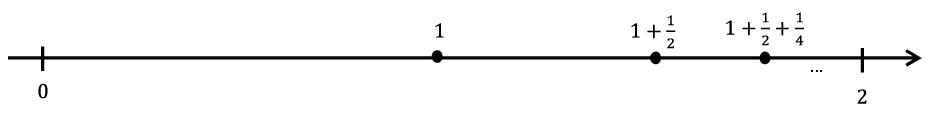
\includegraphics[width=\linewidth]{external/images/NumberLine.png}
			\end{image}%
			Since each partial sum is located at the midpoint between the previous partial sum and \(2\), it is reasonable to suppose that these sums tend to the number 2. Indeed, you probably have seen an expression such as \(\lim_{n\rightarrow\infty}\) \(\left(\sum_{j=0}^n\left(\frac{1}{2}\right)^j\right)=2\) justified by a similar argument. Of course, the reliance on such pictures and words is fine if we are satisfied with intuition. However, we must be able to make these intuitions rigorous without relying on pictures or nebulous words such as ``approaches.''%
			\par
			No doubt you are wondering ``What's wrong with the word `approaches'? It seems clear enough to me.'' This is often a sticking point. But if we think carefully about what we mean by the word ``approach'' we see that there is an implicit assumption that will cause us some difficulties later if we don't expose it.%
			\par
			To see this consider the sequence \(\left(1,\frac12,\frac13,\frac14,\ldots\right)\). Clearly it ``approaches'' zero, right? But, doesn't it also ``approach'' \(-1?\) It does, in the sense that each term gets closer to \(-1\) than the one previous. But it also ``approaches'' \(-2\), \(-3\), or even \(-1000\) in the same sense. That's the problem with the word ``approaches.'' It just says that we're getting closer to something than we were in the previous step. It does \emph{not} tell us that we are actually getting close. Since the moon moves in an elliptical orbit about the earth for part of each month it is ``approaching'' the earth. The moon gets clos\emph{er} to the earth but, thankfully, it does not get \emph{close} to the earth. The implicit assumption we alluded to earlier is this: When we say that the sequence \(\left(\frac1n\right)_{n=1}^\infty\) ``approaches'' zero we mean that it is getting \emph{close} not clos\emph{er}. Ordinarily this kind of vagueness in our language is pretty innocuous. When we say ``approaches'' in casual conversation we can usually tell from the context of the conversation whether we mean ``getting close to'' or ``getting closer to.'' But when speaking mathematically we need to be more careful, more explicit, in the language we use.%
			\par
			So how can we change the language we use so that this ambiguity is eliminated? Let's start out by recognizing, rigorously, what we mean when we say that a sequence converges to zero. For example, you would probably want to say that the sequence \(\left(1,\frac{1}{2},\frac{1}{3},\frac{1}{4},\,\ldots\right)=\left( \frac{1}{n}\right)_{n=1}^\infty\) converges to zero. Is there a way to give this meaning without relying on pictures or intuition?%
			\par
			One way would be to say that we can make \(\frac{1}{n}\) as close to zero as we wish, provided we make \(n\) large enough. But even this needs to be made more specific. For example, we can get \(\frac{1}{n}\) to within a distance of \(.1\) of \(0\) provided we make \(n>10\), we can get \(\frac{1}{n}\) to within a distance of \(.01\) of \(0\) provided we make \(n>100\), etc. After a few such examples it is apparent that given any arbitrary distance \(\eps>0\), we can get \(\frac{1}{n}\) to within \(\eps\) of \(0\) provided we make \(n>\frac{1}{\eps}\). This leads to the following definition.%
			\begin{definition}{}{x:definition:def_ConvergeToZero}%
				\index{sequences!convergence to zero} Let \(\left(s_n\right)=\left(s_1,s_2,s_3,\ldots\right)\) be a sequence of real numbers. We say that \(\left(\boldsymbol{s}_{\boldsymbol{n}}\right)\) \terminology{converges to 0} and write \(\lim_{n\rightarrow\infty}s_n=0\) provided for any \(\eps>0\), there is a real number \(N\) such that if \(n>N\), then \(|s_n|\lt \eps\).%
			\end{definition}
			\terminology{Notes on \hyperref[x:definition:def_ConvergeToZero]{Definition~{\xreffont\ref{x:definition:def_ConvergeToZero}}}}:%
			\begin{enumerate}
				\item{}This definition is the formal version of the idea we just talked about; that is, given an arbitrary distance \(\eps\), we must be able to find a specific number \(N\) such that \(s_n\) is within \(\eps\) of \(0\), whenever \(n>N\). The \(N\) is the answer to the question of how large is ``large enough'' to put \(s_n\) this close to \(0\).%
				\item{}Even though we didn't need it in the example \(\left(\frac{1}{n}\right)\), the absolute value appears in the definition because we need to make the \emph{distance} from \(s_n\) to 0 smaller than \(\eps\). Without the absolute value in the definition, we would be able to ``prove'' such outrageous statements as \(\lim_{n\rightarrow\infty}-n=0\), which we obviously don't want.%
				\item{}The statement \(|s_n|\lt \eps\) can also be written as \(-\eps\lt s_n\lt \eps\) or \(s_n\in\left(-\eps,\eps\right)\). (See the \hyperref[x:problem:prob_absolute_value]{Problem~{\xreffont\ref{x:problem:prob_absolute_value}}} below.) Any one of these equivalent formulations can be used to prove convergence. Depending on the application, one of these may be more advantageous to use than the others.%
				\item{}Any time an \(N\) can be found that works for a particular \(\eps\), any number \(M>N\) will work for that \(\eps\) as well, since if \(n>M\) then \(n>N\).%
			\end{enumerate}
			%
			\begin{problem}{}{x:problem:prob_absolute_value}%
				\index{absolute value} Let \(a\) and \(b\) be real numbers with \(b>0\). Prove \(|a|\lt b\) if and only if \(-b\lt a\lt b\). Notice that this can be extended to \(|a|\leq b\) if and only if \(-b\leq a\leq b\).%
			\end{problem}
			To illustrate how this definition makes the above ideas rigorous, let's use it to prove that \(\displaystyle\lim_{n\rightarrow\infty}\frac{1}{n}=0\).%
			\begin{proof}{}{g:proof:idp105}
				Let \(\eps>0\) be given. Let \(N=\frac{1}{\eps}\). If \(n>N\), then \(n>\frac{1}{\eps}\) and so \(|\frac{1}{n}|=\frac{1}{n}\lt \eps\). Hence by definition, \(\lim_{n\rightarrow\infty}\frac{1}{n}=0\).%
			\end{proof}
			Notice that this proof is rigorous and makes no reference to vague notions such as ``getting smaller'' or ``approaching infinity.'' It has three components:%
			\begin{enumerate}
				\item{}provide the challenge of a distance \(\eps>0\),%
				\item{}identify a real number \(N\), and%
				\item{}show that this \(N\) works for this given \(\eps\).%
			\end{enumerate}
			There is also no explanation about where \(N\) came from. While it is true that this choice of \(N\) is not surprising in light of the ``scrapwork'' we did before the definition, the motivation for how we got it is not in the formal proof nor is it required.  In fact, such scrapwork is typically not included in a formal proof.  For example, consider the following.%
			\begin{example}{}{g:example:idp106}%
				Use the definition of convergence to zero to prove%
				\begin{equation*}
					\lim_{n\rightarrow\infty}\frac{\sin n}{n}=0\text{.}
				\end{equation*}
				%
			\end{example}
			\begin{proof}{}{g:proof:idp107}
				Let \(\eps>0\). Let \(N=\frac{1}{\eps}\). If \(n>N\), then \(n>\frac{1}{\eps}\) and \(\frac{1}{n}\lt \eps\). Thus \(\abs{\frac{\sin(n)}{n}}\leq\frac{1}{n}\lt \eps\). Hence by definition, \(\lim_{n\rightarrow\infty}\frac{\sin n}{n}=0\).%
			\end{proof}
			Notice that the \(N\) came out of nowhere, but you can probably see the thought process that went into this choice: We needed to use the inequality \(\abs{\sin n}\leq 1\). Again this scrapwork is not part of the formal proof, but it is typically necessary for finding what \(N\) should be. You might be able to do the next problem without doing any scrapwork first, but don't hesitate to do scrapwork if you need it.%
			\begin{problem}{}{g:problem:idp108}%
				\index{convergence!of a sequence!convergence to zero drill} Use the definition of convergence to zero to prove the following.%
				\begin{enumerate}[font=\bfseries,label=(\alph*),ref=\alph*]
					\item{}\(\displaystyle\lim_{n\rightarrow\infty}\frac{1}{n^2}=0\)%
					\item{}\(\displaystyle\lim_{n\rightarrow\infty}\frac{1}{\sqrt{n}}=0\)%
				\end{enumerate}
			\end{problem}
			As the sequences get more complicated, doing scrapwork ahead of time will become more necessary.%
			\begin{example}{}{x:example:sec_defin-conv-sequ}%
				Use the definition of convergence to zero to prove%
				\begin{equation*}
					\lim_{n\rightarrow\infty}\frac{n+4}{n^2+1}=0\text{.}
				\end{equation*}
				%
				\par
				\terminology{SCRAPWORK}%
				\par
				Given an \(\eps>0\), we need to see how large to make \(n\) in order to guarantee that \(|\frac{n+4}{n^2+1}|\lt \eps\). First notice that \(\frac{n+4}{n^2+1}\lt \frac{n+4}{n^2}\). Also, notice that if \(n>4\), then \(n+4\lt n+n=2n\). So as long as \(n>4\), we have \(\frac{n+4}{n^2+1}\lt \frac{n+4}{n^2}\lt \frac{2n}{n^2}=\frac{2}{n}\). We can make this less than \(\eps\) if we make \(n>\frac{2}{\eps}\). This means we need to make \(n>4\) and \(n>\frac{2}{\eps}\), simultaneously. These can be done if we let \(N\) be the maximum of these two numbers. This sort of thing comes up regularly, so the notation \(N=\max\left(4,\frac{2}{\eps}\right)\) was developed to mean the maximum of these two numbers. Notice that if \(N=\max\left(4, \frac{2}{\eps}\right)\) then \(N\geq 4\) and \(N\geq\frac{2}{\eps}\). We're now ready for the formal proof.%
			\end{example}
			\begin{proof}{}{g:proof:idp109}
				Let \(\eps>0\). Let \(N=\max\left(4,\frac{2}{\eps}\right)\). If \(n>N\), then \(n>4\) and \(n>\frac{2}{\eps}\). Thus we have \(n>4\) and \(\frac{2}{n}\lt \eps\). Therefore%
				\begin{equation*}
					\abs{\frac{n+4}{n^2+1}}=\frac{n+4}{n^2+1}\lt \frac{n+4}{n^2}\lt \frac{2n}{n^2}= \frac{2}{n}\lt \eps\text{.}
				\end{equation*}
				%
				\par
				Hence by definition, \(\displaystyle\lim_{n\rightarrow\infty}\frac{n+4}{n^2+1}=0\).%
			\end{proof}
			Again we emphasize that the scrapwork is not \alert{explicitly} a part of the formal proof.  However, if you look carefully, you can always find the scrapwork in the formal proof.%
			\begin{problem}{}{g:problem:idp110}%
				\index{convergence!of a sequence!convergence to zero drill} Use the definition of convergence to zero to prove%
				\begin{equation*}
					\lim_{n\rightarrow\infty}\frac{n^2+4n+1}{n^3}=0.{}
				\end{equation*}
				%
			\end{problem}
			\begin{problem}{}{x:problem:prob_sequences3}%
				Let \(b\) be a nonzero real number with \(|b|\lt 1\) and let \(\eps>0\).%
				\begin{enumerate}[font=\bfseries,label=(\alph*),ref=\alph*]
					\item{}Solve the inequality \(|b|^n\lt \eps\) for \(n\)%
					\item{}Use part (a) to prove \(\lim_{n\rightarrow\infty}b^n=0\).%
				\end{enumerate}
			\end{problem}
			We can negate this definition to prove that a particular sequence does not converge to zero.%
			\begin{example}{}{x:example:ex_zero-two-not-converge}%
				Use the definition to prove that the sequence%
				\begin{equation*}
					\left(1+(-1)^n\right)_{n=0}^\infty=(2,0,2,0,2,\ldots)
				\end{equation*}
				does not converge to zero.%
			\end{example}
			Before we provide this proof, let's analyze what it means for a sequence \(\left(s_n\right)\) to \emph{not} converge to zero.  Converging to zero means that any time a distance \(\eps>0\) is given, we must be able to respond with a number \(N\) such that \(|s_n|\lt \eps\) for every \(n>N\).  To have this not happen, we must be able to find some \(\eps>0\) such that no choice of \(N\) will work.  Of course, if we find such an \(\eps\), then any smaller one will fail to have such an \(N\), but we only need one to mess us up.  If you stare at the example long enough, you see that any \(\eps\) with \(0\lt
			\eps\leq 2\) will cause problems.  For our purposes, we will let \(\eps=2\).%
			\begin{proof}{}{g:proof:idp111}
				Let \(\eps=2\) and let \(N\in\NN\) be any integer. If we let \(k\) be any non-negative integer with \(k>\frac{N}{2}\), then \(n=2k>N\), but \(|1+(-1)^n|=2\). Thus no choice of \(N\) will satisfy the conditions of the definition for this \(\eps\), (namely that \(|1+(-1)^n|\lt 2\) for all \(n>N\)) and so \(\lim_{n\rightarrow\infty}\left(1+(-1)^n\right)\neq 0\).%
			\end{proof}
			\begin{problem}{}{x:problem:prob_sequences-not_converge_to_zero}%
				\index{limit!definition of non-existence} Negate the definition of \(\lim_{n\rightarrow\infty}s_n=0\) to provide a formal definition for \(\lim_{n\rightarrow\infty}s_n\neq 0\).%
			\end{problem}
			\begin{problem}{}{x:problem:prob_sequences4}%
				Use the definition to prove \(\lim_{n\rightarrow\infty}\frac{n}{n+100}\neq 0\).%
			\end{problem}
			Now that we have a handle on how to rigorously prove that a sequence converges to zero, let's generalize this to a formal definition for a sequence converging to something else. Basically, we want to say that a sequence \(\left(s_n\right)\) converges to a real number \(s\), provided the difference \(\left(s_n-s\right)\) converges to zero. This leads to the following definition:%
			\begin{definition}{}{x:definition:def_ConvergenceOfASequence}%
				\index{sequences!convergence}\index{convergence!of a sequence} Let \(\left(s_n\right)=\left(s_1,s_2,s_3,\ldots\right)\) be a sequence of real numbers and let \(s\) be a real number. We say that \(\left(\boldsymbol{s}_{\boldsymbol{n}}\right)\) \textbraceleft{}converges to\textbraceright{} \(\boldsymbol{s}\) and write \(\lim_{n\rightarrow\infty}s_n=s\) provided for any \(\eps>0\), there is a real number \(N\) such that if \(n>N\), then \(|s_n-s|\lt \eps\).%
			\end{definition}
			\textbraceleft{}Notes on \hyperref[x:definition:def_ConvergenceOfASequence]{Definition~{\xreffont\ref{x:definition:def_ConvergenceOfASequence}}}\textbraceright{}%
			\par
			%
			\begin{enumerate}
				\item{}Clearly%
				\begin{equation*}
					\lim_{n\rightarrow\infty}s_n=s \text{ if and only if } \lim_{n\rightarrow\infty}\left(s_n-s\right)=0\text{.}
				\end{equation*}
				%
				\item{}Again notice that this says that we can make \(s_n\) as close to \(s\) as we wish (within \(\eps\)) by making \(n\) large enough (\(>N)\). As before, this definition makes these notions very specific.%
				\item{}Notice that \(|s_n-s|\lt \eps\) can be written in the following equivalent forms%
				\par
				%
				\begin{enumerate}
					\item{}\(\displaystyle |s_n-s|\lt \eps\)%
					\item{}\(\displaystyle -\eps\lt s_n-s\lt \eps\)%
					\item{}\(\displaystyle s-\eps\lt s_n\lt s+\eps\)%
					\item{}\(\displaystyle s_n\in\left(s-\eps,s+\eps\right)\)%
				\end{enumerate}
				%
				\par
				and we are free to use any one of these which is convenient at the time.%
			\end{enumerate}
			%
			\par
			As an example, let's use this definition to prove that the sequence in \hyperref[x:problem:prob_sequences4]{Problem~{\xreffont\ref{x:problem:prob_sequences4}}}, in fact, converges to 1.%
			\begin{example}{}{x:example:example_SeriesConverge}%
				Prove \(\displaystyle\lim_{n\rightarrow\infty}\frac{n}{n+100}=1\).%
				\par
				\terminology{SCRAPWORK}%
				\par
				Given an \(\eps>0\), we need to get \(\abs{\frac{n}{n+100}-1}\lt \eps\). This prompts us to do some algebra.%
				\begin{equation*}
					\left|\frac{n}{n+100}-1\right|=\left|\frac{n-(n+100)}{n+100}\right|\leq\frac{100}{n}\text{.}
				\end{equation*}
				%
				\par
				This in turn, seems to suggest that \(N=\frac{100}{\eps}\) should work.%
			\end{example}
			\begin{proof}{}{g:proof:idp112}
				Let \(\eps>0\). Let \(N=\frac{100}{\eps}\). If \(n>N\), then \(n>\frac{100}{\eps}\) and so \(\frac{100}{n}\lt \eps\). Hence%
				\begin{equation*}
					\left|\frac{n}{n+100}-1\right|=\left|\frac{n-(n+100)}{n+100}\right|= \frac{100}{n+100}\lt \frac{100}{n}\lt \eps\text{.}
				\end{equation*}
				%
				\par
				Thus by definition \(\lim_{n\rightarrow\infty}\frac{n}{n+100} =1\).%
			\end{proof}
			Notice again that the scrapwork is not part of the formal proof and the author of a proof is not obligated to tell where the choice of \(N\) came from (although the thought process can usually be seen in the formal proof). The formal proof contains only the requisite three parts: provide the challenge of an arbitrary \(\eps>0\), provide a specific \(N\), and show that this \(N\) works for the given \(\eps\).%
			\par
			Also notice that given a specific sequence such as \(\left(\frac{n}{n+100}\right)\), the definition does not indicate what the limit would be if, in fact, it exists. Once an educated guess is made as to what the limit should be, the definition only verifies that this intuition is correct.%
			\par
			This leads to the following question: If intuition is needed to determine what a limit of a sequence should be, then what is the purpose of this relatively non-intuitive, complicated definition?%
			\par
			Remember that when these rigorous formulations were developed, intuitive notions of convergence were already in place and had been used with great success. This definition was developed to address the foundational issues. Could our intuitions be verified in a concrete fashion that was above reproach? This was the purpose of this non-intuitive definition. It was to be used to verify that our intuition was, in fact, correct and do so in a very prescribed manner. For example, if \(b>0\) is a fixed number, then you would probably say as \(n\) approaches infinity, \(b^{\left(\frac{1}{n}\right)}\) approaches \(b^0=1\). After all, we did already prove that \(\lim_{n\rightarrow\infty}\frac{1}{n}=0\). We should be able to back up this intuition with our rigorous definition.%
			\begin{problem}{}{g:problem:idp113}%
				\index{limit!\(\lim_{n\rightarrow\infty}b^{\left(\frac{1}{n}\right)}=1\) if \(b>0\)} Let \(b>0\). Use the definition to prove \(\limit{n}{\infty}{b^{\left(\frac{1}{n}\right)}}=1\).%
				\par\smallskip%
				\noindent\textbf{\blocktitlefont Hint}.\hypertarget{g:hint:idp114}{}\quad{}You will probably need to separate this into two cases: \(0\lt b\lt 1\) and \(b\geq 1\).%
			\end{problem}
			\begin{problem}{}{g:problem:idp115}%
				\begin{enumerate}[font=\bfseries,label=(\alph*),ref=\alph*]
					\item{}Provide a rigorous definition for \(\limit{n}{\infty}{s_n}\neq s\).%
					\item{}Use your definition to show that for any real number \(a\), \(\limit{n}{\infty}{\left(\left(-1\right)^n\right)}\neq a\).%
					\par\smallskip%
					\noindent\textbf{\blocktitlefont Hint}.\hypertarget{g:hint:idp116}{}\quad{}Choose \(\eps=1\) and use the fact that \(\Big|a-(-1)^n\Big|\lt 1\) is equivalent to \(\left(-1\right)^n-1\lt a\lt \left(-1\right)^n+1\) to show that no choice of \(N\) will work for this \(\eps\).%
				\end{enumerate}
			\end{problem}
		\end{sectionptx}
		%
		%
		\typeout{************************************************}
		\typeout{Section 7.2 The Limit as a Primary Tool}
		\typeout{************************************************}
		%
		\begin{sectionptx}{The Limit as a Primary Tool}{}{The Limit as a Primary Tool}{}{}{x:section:LimitAsPrimary}
			As you've seen from the previous sections, the formal definition of the convergence of a sequence is meant to capture rigorously our intuitive understanding of convergence. However, the definition itself is an unwieldy tool. If only there was a way to be rigorous without having to run back to the definition each time. Fortunately, there is a way. If we can use the definition to prove some general rules about limits then we could use these rules whenever they applied and be assured that everything was still rigorous. A number of these should look familiar from calculus.%
			\begin{problem}{}{g:problem:idp117}%
				\index{limit!of a constant sequence}\index{sequences!constant sequences} Let \(\left(c\right)_{n=1}^\infty=(c,c,c,\ldots)\) be a constant sequence. Show that \(\lim_{n\rightarrow\infty}c=c\).%
			\end{problem}
			In proving the familiar limit theorems, the following will prove to be a very useful tool.%
			\begin{lemma}{}{}{x:lemma:Tri-RevTri-Ineq}%
				\index{Triangle Inequalities}%
				%
				\begin{descriptionlist}
					\begin{dlimedium}{Triangle Inequality:}{x:li:TriangleIneq}%
						\index{Triangle Inequalities!Triangle Inequality}Let \(a\) and \(b\) be real numbers. Then%
						\begin{equation*}
							|a+b|\leq|a|+|b|\text{.}
						\end{equation*}
						%
					\end{dlimedium}%
					\begin{dlimedium}{Reverse Triangle Inequality:}{x:li:InvTriangleIneq}%
						\index{Triangle Inequalities!Reverse Triangle Inequalitiy}Let \(a\) and \(b\) be real numbers. Then%
						\begin{equation*}
							|a|-|b|\leq\abs{a-b} {}
						\end{equation*}
						%
					\end{dlimedium}%
				\end{descriptionlist}
				%
			\end{lemma}
			\begin{problem}{}{x:problem:Tri-RevTri-Ineq_prob}%
				\begin{enumerate}[font=\bfseries,label=(\alph*),ref=\alph*]
					\item{}Prove \hyperref[x:lemma:Tri-RevTri-Ineq]{Lemma~{\xreffont\ref{x:lemma:Tri-RevTri-Ineq}}}.%
					\par\smallskip%
					\noindent\textbf{\blocktitlefont Hint}.\hypertarget{g:hint:idp118}{}\quad{}For the Reverse Triangle Inequality, consider \(|a|=|a-b+b|\).%
					\item{}Show \(||a|-|b||\leq|a-b|\).%
					\par\smallskip%
					\noindent\textbf{\blocktitlefont Hint}.\hypertarget{g:hint:idp119}{}\quad{}You want to show \(|a|-|b|\leq|a-b|\) and \(-(|a|-|b|)\leq|a-b|\).%
				\end{enumerate}
			\end{problem}
			\begin{theorem}{}{}{x:theorem:thm_SumOfSequences}%
				\index{limit!termwise sums of} If \(\displaystyle\lim_{n\rightarrow\infty}a_n=a\) and \(\displaystyle\lim_{n\rightarrow\infty}b_n=b\), then \(\displaystyle\lim_{n\rightarrow\infty}\left(a_n+b_n\right)=a+b\).%
			\end{theorem}
			We will often informally state this theorem as ``the limit of a sum is the sum of the limits.'' However, to be absolutely precise, what it says is that if we already know that two sequences converge, then the sequence formed by summing the corresponding terms of those two sequences will converge and, in fact, converge to the sum of those individual limits. We'll provide the scrapwork for the proof of this and leave the formal write-up as an exercise. Note the use of the triangle inequality in the proof.%
			\par
			%
			\begin{problem}{}{g:problem:idp120}%
				\index{sequences!termwise sums of} Prove \hyperref[x:theorem:thm_SumOfSequences]{Theorem~{\xreffont\ref{x:theorem:thm_SumOfSequences}}}.%
				\par
				\terminology{SCRAPWORK:}%
				\par
				If we let \(\eps>0\), then we want \(N\) so that if \(n>N\), then \(\big|\left(a_n+b_n\right)-\left(a+b\right)\big|\lt \eps\). We \emph{know} that \(\limit{n}{\infty}{a_n}=a\) and \(\limit{n}{\infty}{b_n}=b\), so we can make \(\big|a_n-a\big|\) and  \(\big|b_n-b\big|\) as small as we wish, provided we make \(n\) large enough. Let's go back to what we want, to see if we can close the gap between what we know and what we want.%
				\begin{equation*}
					\left|\left(a_n+b_n\right)-\left(a+b\right)\right|=\left|\left(a_n-a\right)+\left(b_n-b\right)\right|\leq\left|a_n-a\right|+\left|b_n-b\right|
				\end{equation*}
				by the triangle inequality. To make this whole thing less than \(\eps\), it makes sense to make each part less than \(\frac{\eps}{2}\). it makes sense to make each part less than \(\frac{\eps}{2}\). Fortunately, we can do that as the definitions of \(\limit{n}{\infty}{a_n}=a\) and \(\limit{n}{\infty}{b_n}=b\) allow us to make \(\big|a_n-a\big|\) and \(\big|b_n-b\big|\) arbitrarily small. Specifically, since \(\limit{n}{\infty}{a_n}=a\), there exists an \(N_1\) such that if \(n>N_1\) then \(\big|a_n-a\big|\lt \frac{\eps}{2}\). Also since \(\limit{n}{\infty}{b_n}=b\), there exists an \(N_2\) such that if \(n>N_2\) then \(\big|b_n-b\big|\lt \frac{\eps}{2}\). Since we want both of these to occur, it makes sense to let \(N=\)max\(\left(N_1,N_2\right)\). This should be the \(N\) that we seek.%
			\end{problem}
			\begin{theorem}{}{}{x:theorem:thm_LimitOfProduct}%
				\index{limit!products of} If \(\displaystyle\lim_{n\rightarrow\infty}a_n=a\) and \(\displaystyle\lim_{n\rightarrow\infty}b_n=b\), then \(\displaystyle\lim_{n\rightarrow\infty}\left(a_n b_n\right)=a b\).%
			\end{theorem}
			\terminology{SCRAPWORK:} Given \(\eps>0\), we want \(N\) so that if \(n>N\), then \(\big|a_n  b_n-a  b\big|\lt \eps\). One of the standard tricks in analysis is to ``uncancel.'' In this case we will subtract and add a convenient term. Normally these would ``cancel out,'' which is why we say that we will uncancel to put them back in. You already saw an example of this in proving the Reverse Triangle Inequality (\hyperref[x:problem:Tri-RevTri-Ineq_prob]{Problem~{\xreffont\ref{x:problem:Tri-RevTri-Ineq_prob}}}). In the present case, consider%
			\begin{align*}
				\left|a_n  b_n-a  b\right|\amp =\left|a_n  b_n-a_n b+a_n b-a  b\right|\\
				\amp \leq\left|a_n  b_n-a_n  b\right|+\left|a_n b-a b\right|\\
				\amp =\left|a_n\right|\left|b_n-b\right|+\left|b\right|\left|a_n-a\right|\text{.}
			\end{align*}
			%
			\par
			We can make this whole thing less than \(\eps\), provided we make each term in the sum less than \(\frac{\eps}{2}\). We can make \(\big|b\big|\big|a_n-a\big|\lt \frac{\eps}{2}\) if we make \(\big|a_n-a\big|\lt \frac{\eps}{2|b|}\). But wait! What if \(b=0\)? We could handle this as a separate case or we can do the following ``slick trick.'' Notice that we can add one more line to the above string of inequalities: \(\left|a_n\right|\left|b_n-b\right|+\left|b\right|\left|a_n-a\right|\lt \left|a_n \right|\left|b_n-b\right|+\left(\left|b\right|+1\right)\left|a_n-a \right|\). Now we can make \(\left|a_n-a\right|\lt \frac{\eps}{2\left(|b|+1\right)}\) and not worry about dividing by zero.%
			\par
			Making \(\big|a_n\big|\big|b_n-b\big|\lt \frac{\eps}{2}\) requires a bit more finesse. At first glance, one would be tempted to try and make \(\big|b_n-b\big|\lt \frac{\eps}{2|a_n|}\). Even if we ignore the fact that we could be dividing by zero (which we could handle), we have a bigger problem. According to the definition of \(\lim_{n\rightarrow\infty}b_n=b\), we can make \(\big|b_n-b\big|\) smaller than any given fixed positive number, as long as we make \(n\) large enough (larger than some \(N\) which goes with a given epsilon). Unfortunately, \(\frac{\eps}{2|a_n|}\) is not fixed as it has the variable \(n\) in it; there is no reason to believe that a single \(N\) will work with all of these simultaneously. To handle this impasse, we need the following:%
			\begin{lemma}{}{}{x:lemma:lemma_BoundedConvergent}%
				\index{sequences!convergence of!convergent sequences are bounded}%
				\alert{A Convergent Sequence Is Bounded.}%
				\par
				If \(\lim_{n\rightarrow\infty}a_n=a\), then there exists \(B>0\) such that \(|a_n|\leq B\) for all \(n\).%
			\end{lemma}
			\begin{problem}{}{x:problem:prob_BoundedConvergent}%
				Prove \hyperref[x:lemma:lemma_BoundedConvergent]{Lemma~{\xreffont\ref{x:lemma:lemma_BoundedConvergent}}}.%
				\par\smallskip%
				\noindent\textbf{\blocktitlefont Hint}.\hypertarget{g:hint:idp121}{}\quad{}We know that there exists \(N\) such that if \(n>N\), then \(\abs{a_n-a}\lt 1\).  Let \(B=\)max\(\left(\abs{a_1},\abs{a_2},\ldots,\abs{a_{\lceil{N}\rceil}},\abs{a}+1\right)\), where \(\lceil{N}\rceil\) represents the smallest integer greater than or equal to \(N\).  Also, notice that this is not a convergence proof so it is not safe to think of \(N\) as a large number.%
				\begin{aside}{}{g:aside:idp122}%
					Actually, this is a dangerous habit to fall into even in convergence proofs.%
				\end{aside}
			\end{problem}
			Armed with this bound \(B\), we can add on one more inequality to the above scrapwork to get%
			\begin{align*}
				\left|a_n\cdot b_n-a\cdot b\right|\amp =\left|a_n\cdot b_n-a_n\cdot b+a_n\cdot b-a\cdot b\right|\\
				\amp \leq\left|a_n\cdot b_n-a_n\cdot b\right|+\left|a_n\cdot b-a\cdot b\right|\\
				\amp =\left|a_n\right|\left|b_n-b\right|+\left|b\right|\left|a_n-a\right|\\
				\amp \lt B\left|b_n-b\right|+\left(\left|b\right|+1\right)\left|a_n-a\right|
			\end{align*}
			%
			\par
			At this point, we should be able to make the last line of this less than \(\eps\).%
			\par
			\terminology{END OF SCRAPWORK}%
			\begin{problem}{}{g:problem:idp123}%
				\index{sequences!termwise product of} Prove \hyperref[x:theorem:thm_LimitOfProduct]{Theorem~{\xreffont\ref{x:theorem:thm_LimitOfProduct}}}.%
			\end{problem}
			\begin{corollary}{}{}{x:corollary:cor_1}%
				(Corollary to \hyperref[x:theorem:thm_LimitOfProduct]{Theorem~{\xreffont\ref{x:theorem:thm_LimitOfProduct}}}) If \(\displaystyle\lim_{n\rightarrow\infty}a_n=a\) and \(c\in\mathbb{R}\), then \(\displaystyle\lim_{n\rightarrow\infty}c\cdot a_n=c\cdot a\).%
			\end{corollary}
			\begin{problem}{}{g:problem:idp124}%
				\index{sequences!constant multiples of}\index{limit!of a constant times a sequence} Prove  \hyperref[x:corollary:cor_1]{Corollary~{\xreffont\ref{x:corollary:cor_1}}}.%
			\end{problem}
			Just as \hyperref[x:theorem:thm_LimitOfProduct]{Theorem~{\xreffont\ref{x:theorem:thm_LimitOfProduct}}} says that the limit of a product is the product of the limits, we can prove the analogue for quotients.%
			\begin{theorem}{}{}{x:theorem:thm_LimitOfQuotient}%
				\index{limit!quotients of} Suppose \(\displaystyle\lim_{n\rightarrow\infty}a_n=a\) and \(\displaystyle\lim_{n\rightarrow\infty}b_n=b\). Also suppose \(b\neq 0\) and \(b_n\neq 0,\forall\,n\). Then \(\displaystyle\lim_{n\rightarrow\infty}\left(\frac{a_n}{b_n}\right)=\frac{a}{b}\).%
			\end{theorem}
			\begin{problem}{}{g:problem:idp125}%
				\index{sequences!termwise quotient of} Prove \hyperref[x:theorem:thm_LimitOfQuotient]{Theorem~{\xreffont\ref{x:theorem:thm_LimitOfQuotient}}}.%
				\par
				\terminology{SCRAPWORK}%
				\par
				To prove this, let's look at the special case of trying to prove \(\lim_{n\rightarrow\infty}\left(\frac{1}{b_n}\right)=\frac{1}{b}\). The general case will follow from this and \hyperref[x:theorem:thm_LimitOfProduct]{Theorem~{\xreffont\ref{x:theorem:thm_LimitOfProduct}}}. Consider \(\big|\frac{1}{b_n}-\frac{1}{b}\big|=\frac{|b-b_n|}{|b_n||b|}\). We are faced with the same dilemma as before; we need to get \(\big|\frac{1}{b_n}\big|\) bounded above. This means we need to get \(|b_n|\) bounded away from zero (at least for large enough \(n\)).%
				\par
				This can be done as follows. Since \(b\neq 0\), then \(\frac{|b|}{2}>0\). Thus, by the definition of \(\lim_{n\rightarrow\infty}b_n=b\) , there exists \(N_1\) such that if \(n>N_1\), then \(|b\mathopen|-|b_n|\leq\big|b-b_n\big|\lt \frac{|b|}{2}\). Thus when \(n>N_1\), \(\frac{|b|}{2}\lt |b_n|\) and so \(\frac{1}{|b_n|}\lt \frac{2}{|b|}\). This says that for \(n>N_1\), \(\frac{|b-b_n|}{|b_n||b|}\lt \frac{2}{|b|^2}|b-b_n|\). We should be able to make this smaller than a given \(\eps>0\), provided we make \(n\) large enough.%
			\end{problem}
			These theorems allow us to compute limits of complicated sequences and rigorously verify that these are, in fact, the correct limits without resorting to the definition of a limit.%
			\begin{problem}{}{g:problem:idp126}%
				\index{limit!identifing the theorems used in a limit} Identify all of the theorems implicitly used to show that%
				\begin{equation*}
					\lim_{n\rightarrow\infty}\frac{3n^3-100n+1}{5n^3+4n^2-7}=\lim_{n \rightarrow\infty}\frac{n^3\left(3-\frac{100}{n^2}+\frac{1}{n^3}\right)}{n^3 \left(5+\frac{4}{n}-\frac{7}{n^3}\right)}=\frac{3}{5}\text{.}
				\end{equation*}
				%
				\par
				Notice that this presumes that all of the individual limits exist. This will become evident as the limit is decomposed.%
			\end{problem}
			There is one more tool that will prove to be valuable.%
			\begin{theorem}{}{}{x:theorem:thm_SqueezeTheorem}%
				\index{limit!Squeeze Theorem for Sequences}%
				\terminology{Squeeze Theorem for Sequences}%
				\par
				Let \(\left(r_n\right),\left(s_n\right)\), and \(\left(t_n\right)\) be sequences of real numbers with \(r_n\leq s_n\leq t_n,\forall\) positive integers \(n\). Suppose \(\lim_{n\rightarrow\infty}r_n=s=\lim_{n\rightarrow\infty}t_n\). Then \(\left(s_n\right)\) must converge and \(\lim_{n\rightarrow\infty}s_n=s\).%
			\end{theorem}
			\begin{problem}{}{g:problem:idp127}%
				Prove \hyperref[x:theorem:thm_SqueezeTheorem]{Theorem~{\xreffont\ref{x:theorem:thm_SqueezeTheorem}}}.%
				\par\smallskip%
				\noindent\textbf{\blocktitlefont Hint}.\hypertarget{g:hint:idp128}{}\quad{}This is probably a place where you would want to use \(s-\eps\lt s_n\lt s+\eps\) instead of \(|s_n-s|\lt
				\eps\).%
			\end{problem}
			The Squeeze Theorem holds even if \(r_n\leq s_n\leq t_n\) holds for only sufficiently large \(n\); i.e., for \(n\) larger than some fixed \(N_0\). This is true because when you find an \(N_1\) that works in the original proof, this can be modified by choosing \(N=\)max\(\left(N_0,N_1\right)\). Also note that this theorem really says two things: \(\left(s_n\right)\) converges and it converges to \(s\). This subtle point affects how one should properly use the Squeeze Theorem.%
			\begin{example}{}{x:example:example_SqzeEx}%
				Prove \(\displaystyle\lim_{n\rightarrow\infty}\frac{n+1}{n^2}=0\).%
			\end{example}
			\begin{proof}{}{g:proof:idp129}
				Notice that \(0\leq\frac{n+1}{n^2}\leq\frac{n+n}{n^2}=\frac{2}{n}\). Since \(\displaystyle\lim_{n\rightarrow\infty}0=0=\lim_{n\rightarrow\infty}\frac{2}{n}\), then by the Squeeze Theorem, \(\displaystyle\lim_{n\rightarrow\infty}\frac{n+1}{n^2}=0\).%
			\end{proof}
			Notice that this proof is completely rigorous. Also notice that this is the proper way to use the Squeeze Theorem. Here is an example of an \textbraceleft{}improper\textbraceright{} use of the Squeeze Theorem.%
			\par
			How \emph{not} to prove \hyperref[x:example:example_SqzeEx]{Example~{\xreffont\ref{x:example:example_SqzeEx}}}. Notice that%
			\begin{equation*}
				0\leq\frac{n+1}{n^2}\leq\frac{n+n}{n^2}=\frac{2}{n}\text{,}
			\end{equation*}
			so%
			\begin{equation*}
				0=\lim_{n\rightarrow\infty}0 \leq \lim_{n\rightarrow\infty}\frac{n+1}{n^2}\leq\lim_{n\rightarrow\infty}\frac{2}{n}=0
			\end{equation*}
			and%
			\begin{equation*}
				\lim_{n\rightarrow\infty}\frac{n+1}{n^2}=0\text{.}
			\end{equation*}
			%
			\par
			This is incorrect in form because it presumes that \(\lim_{n\rightarrow\infty}\frac{n+1}{n^2}\) exists, which we don't yet know. If we knew that the limit existed to begin with, then this would be fine. The Squeeze Theorem proves that the limit does in fact exist, but it must be so stated.%
			\par
			These general theorems will allow us to rigorously explore convergence of power series in the next chapter without having to appeal directly to the definition of convergence. However, you should remember that we used the definition to prove these results and there will be times when we will need to apply the definition directly. However, before we go into that, let's examine divergence a bit more closely.%
		\end{sectionptx}
		%
		%
		\typeout{************************************************}
		\typeout{Section 7.3 Divergence}
		\typeout{************************************************}
		%
		\begin{sectionptx}{Divergence}{}{Divergence}{}{}{x:section:DivergentSeq}
			In \hyperref[x:theorem:thm_rearrangements]{Theorem~{\xreffont\ref{x:theorem:thm_rearrangements}}} we saw that there is a rearrangment of the alternating Harmonic series which diverges to \(\infty\) or \(-\infty\). In that section we did not fuss over any formal notions of divergence. We assumed instead that you are already familiar with the concept of divergence, probably from taking calculus in the past.%
			\par
			However we are now in the process of building precise, formal definitions for the concepts we will be using so we define the divergence of a sequence as follows.%
			\begin{definition}{}{x:definition:thm_divergence_of_a_sequence}%
				\index{sequences!divergence of}\index{divergence!of a sequence} A sequence of real numbers \(\left(s_n\right)_{n=1}^\infty\) diverges if it does not converge to any \(a\in\RR\).%
			\end{definition}
			It may seem unnecessarily pedantic of us to insist on formally stating such an obvious definition. After all ``converge'' and ``diverge'' are opposites in ordinary English. Why wouldn't they be mathematically opposite too? Why do we have to go to the trouble of formally defining both of them? Since they are opposites defining one implicitly defines the other doesn't it?%
			\par
			One way to answer that criticism is to state that in mathematics we \emph{always} work from precisely stated definitions and tightly reasoned logical arguments.%
			\par
			But this is just more pedantry. It is a way of saying, ``Because we said so'' all dressed up in imposing language. We need to do better than that.%
			\par
			One reason for providing formal definitions of both convergence and divergence is that in mathematics we frequently co-opt words from natural languages like English and imbue them with mathematical meaning that is only tangentially related to the original English definition. When we take two such words which happen to be opposites in English and give them mathematical meanings which are \emph{not} opposites it can be very confusing, especially at first.%
			\par
			This is what happened with the words ``open'' and ``closed.'' These are opposites in English: ``not open'' is ``closed,'' ``not closed'' is ``open,'' and there is nothing which is both open and closed. But recall that an open interval on the real line, \((a,b)\), is one that does not include \emph{either} of its endpoints while a closed interval, \([a,b]\), is one that includes both of them.%
			\par
			These may seem like opposites at first but they are not.  To see this observe that the interval \((a,b]\) is neither open nor closed since it only contains one of its endpoints. If ``open'' and ``closed'' were mathematically opposite then \emph{every} interval would be either open or closed.%
			\begin{aside}{Open Sets vs. Closed Sets.}{g:aside:idp130}%
				It is also true that \((-\infty,\infty)\) is \emph{both} open and closed, but an explanation of this would take us too far afield.%
			\end{aside}
			Mathematicians have learned to be extremely careful about this sort of thing. In the case of convergence and divergence of a series, even though these words are actually opposites mathematically (every sequence either converges or diverges and no sequence converges \emph{and} diverges) it is better to say this explicitly so there can be no confusion.%
			\par
			A sequence \(\left(a_n\right)_{n=1}^\infty\) can only converge to a real number, \(a\), in one way: by getting arbitrarily close to \(a\). However there are several ways a sequence might diverge.%
			\begin{example}{}{g:example:idp131}%
				Consider the sequence, \(\left(n\right)_{n=1}^\infty\). This clearly diverges by getting larger and larger \(\ldots\) Ooops! Let's be careful. The sequence \(\left(1-\frac1n\right)_{n=1}^\infty\) gets larger and larger too, but it converges. What we meant to say was that the terms of the sequence \(\left(n\right)_{n=1}^\infty\) become \emph{arbitrarily} large as \(n\) increases.%
				\par
				This is clearly a divergent sequence but it may not be clear how to prove this formally. Here's one way.%
				\par
				To show divergence we must show that the sequence satisfies the \emph{negation} of the definition of convergence. That is, we must show that for every \(r\in\RR\) there is an \(\eps>0\) such that for every \(N\in\RR\), there is an \(n>N\) with \(\left|n-r\right|\ge\eps\).%
				\par
				So let \(\eps=1\), and let \(r\in\RR\) be given. Let \(N=r+2\). Then for every \(n>N\) \(\abs{n-r} > \abs{(r+2)-r}=2>1\). Therefore the sequence diverges.%
			\end{example}
			This seems to have been rather more work than we should have to do for such a simple problem. Here's another way which highlights this particular type of divergence.%
			\par
			First we'll need a new definition:%
			\begin{definition}{}{x:definition:def_DivToInf}%
				\index{sequences!divergence to \(\infty\)}\index{\(\infty\)!positive infinity!divergence to} A sequence, \(\left(a_n\right)_{n=1}^\infty\), \terminology{diverges to positive infinity} if for every real number \(r\), there is a real number \(N\) such that \(n>N\imp a_n>r\).%
				\par
				\index{\(\infty\)!negative infinity!divergence to} A sequence, \(\left(a_n\right)_{n=1}^\infty\), \terminology{diverges to negative infinity} if for every real number \(r\), there is a real number \(N\) such that \(n>N\imp a_n\lt r\).%
				\par
				\index{\(\infty\)!divergence to} A sequence is said to \terminology{diverge to infinity} if it diverges to either positive or negative infinity.%
			\end{definition}
			In practice we want to think of \(\abs{r}\) as a very large number. This definition says that a sequence diverges to infinity if it becomes arbitrarily large as \(n\) increases, and similarly for divergence to negative infinity.%
			\begin{problem}{}{g:problem:idp132}%
				\index{sequences!the sequence of positive integers diverges to infinity} Show that \(\left(n\right)_{n=1}^\infty\) diverges to infinity.%
			\end{problem}
			\begin{problem}{}{g:problem:idp133}%
				\index{sequences!divergence to \(\infty\)}\index{divergence!divergence to infinity implies divergence} Show that if \(\left(a_n\right)_{n=1}^\infty\) diverges to infinity then \(\left(a_n\right)_{n=1}^\infty\) diverges.%
			\end{problem}
			We will denote divergence to infinity as%
			\begin{equation*}
				\limit{n}{\infty}{a_n}=\pm\infty\text{.}
			\end{equation*}
			%
			\par
			However, strictly speaking this is an abuse of notation since the symbol \(\infty\) does not represent a real number. This notation can be very problematic since it looks so much like the notation we use to denote convergence: \(\limit{n}{\infty}{a_n}=a\).%
			\par
			Nevertheless, the notation is appropriate because divergence to infinity is ``nice'' divergence in the sense that it shares many of the properties of convergence, as the next problem shows.%
			\begin{problem}{}{g:problem:idp134}%
				Suppose \(\limit{n}{\infty}{a_n}=\infty\) and \(\limit{n}{\infty}{b_n}=\infty\).%
				\begin{enumerate}[font=\bfseries,label=(\alph*),ref=\alph*]
					\item{}Show that \(\limit{n}{\infty}{a_n+b_n}=\infty\)%
					\item{}Show that \(\limit{n}{\infty}{a_nb_n}=\infty\)%
					\item{}Is it true that \(\limit{n}{\infty}{\frac{a_n}{b_n}}=\infty?\) Explain.%
				\end{enumerate}
			\end{problem}
			Because divergence to positive or negative infinity shares some of the properties of convergence it is easy to get careless with it.  Remember that even though we write \(\limit{n}{\infty}{a_n}=\infty\) this is still a divergent sequence in the sense that \(\limit{n}{\infty}{a_n}\) does not exist.  The symbol \(\infty\) does not represent a real number.  This is just a convenient notational shorthand telling us that the sequence diverges by becoming arbitrarily large.%
			\begin{problem}{}{g:problem:idp135}%
				Suppose \(\limit{n}{\infty}{a_n}=\infty\) and \(\limit{n}{\infty}{b_n}=-\infty\) and \(\alpha\in\RR\).  Prove or give a counterexample:%
				\begin{enumerate}[font=\bfseries,label=(\alph*),ref=\alph*]
					\item{}\(\limit{n}{\infty}{a_n+b_n}=\infty\)%
					\item{}\(\limit{n}{\infty}{a_nb_n}=-\infty\)%
					\item{}\(\limit{n}{\infty}{\alpha a_n}=\infty\)%
					\item{}\(\limit{n}{\infty}{\alpha b_n}=-\infty\)%
				\end{enumerate}
			\end{problem}
			Finally, a sequence can diverge in other ways as the following problem displays.%
			\begin{problem}{}{g:problem:idp136}%
				Show that each of the following sequences diverge.%
				\begin{enumerate}[font=\bfseries,label=(\alph*),ref=\alph*]
					\item{}\(\left(\left(-1\right)^n\right)_{n=1}^\infty\)%
					\item{}\(\left(\left(-1\right)^nn\right)_{n=1}^\infty\)%
					\item{}\(a_n = \begin{cases}1\amp \text{ if \(n=2^p\) for some \(p\in\NN\) } \\ \frac1n\amp \text{ otherwise. } \end{cases}\)%
				\end{enumerate}
			\end{problem}
			\begin{problem}{}{g:problem:idp137}%
				Suppose that \(\left(a_n\right)_{n=1}^\infty\) diverges but not to infinity and that \(\alpha\) is a real number. What conditions on \(\alpha\) will guarantee that:%
				\begin{enumerate}[font=\bfseries,label=(\alph*),ref=\alph*]
					\item{}\(\left(\alpha a_n\right)_{n=1}^\infty\) converges?%
					\item{}\(\left(\alpha a_n\right)_{n=1}^\infty\) diverges?%
				\end{enumerate}
			\end{problem}
			\begin{problem}{}{g:problem:idp138}%
				Show that if \(\abs{r}>1\) then \(\left(r^n\right)_{n=1}^\infty\) diverges. Will it diverge to infinity?%
			\end{problem}
		\end{sectionptx}
		%
		%
		\typeout{************************************************}
		\typeout{Section 7.4 Additional Problems}
		\typeout{************************************************}
		%
		\begin{sectionptx}{Additional Problems}{}{Additional Problems}{}{}{g:section:idp139}
			\begin{problem}{}{g:problem:idp140}%
				Prove that if \(\lim_{n\rightarrow\infty}s_n=s\) then \(\lim_{n\rightarrow\infty}|s_n|=|s|\). Prove that the converse is true when \(s=0\), but it is not necessarily true otherwise.%
			\end{problem}
			\begin{problem}{}{g:problem:idp141}%
				\begin{enumerate}[font=\bfseries,label=(\alph*),ref=\alph*]
					\item{}Let \(\left(s_n\right)\) and \(\left(t_n\right)\) be sequences with \(s_n\leq t_n,\forall n\). Suppose \(\lim_{n\rightarrow\infty}s_n=s\) and \(\lim_{n\rightarrow\infty}t_n=t\).%
					\par
					Prove \(s\leq t\).%
					\par\smallskip%
					\noindent\textbf{\blocktitlefont Hint}.\hypertarget{g:hint:idp142}{}\quad{}Assume for contradiction, that \(s>t\) and use the definition of convergence with \(\eps=\frac{s-t}{2}\) to produce an \(n\) with \(s_n>t_n\).%
					\item{}Prove that if a sequence converges, then its limit is unique.  That is, prove that if \(\lim_{n\rightarrow\infty}s_n=s\) and \(\lim_{n\rightarrow\infty}s_n=t\), then \(s=t\).%
				\end{enumerate}
			\end{problem}
			\begin{problem}{}{g:problem:idp143}%
				Prove that if the sequence \(\left(s_n\right)\) is bounded then \(\lim_{n\rightarrow\infty}\left(\frac{s_n}{n}\right)=0\).%
			\end{problem}
			\begin{problem}{}{x:problem:prob_series-geometric}%
				\begin{enumerate}[font=\bfseries,label=(\alph*),ref=\alph*]
					\item{}Prove that if \(x\neq 1\), then%
					\begin{equation*}
						1+x+x^2+\cdots+x^n=\frac{1-x^{n+1}}{1-x}\text{.}
					\end{equation*}
					%
					\item{}Use (a) to prove that if \(|x|\lt 1\), then \(\lim_{n\rightarrow\infty}\left(\sum_{j=0}^nx^j\right)=\frac{1}{1-x}\).%
				\end{enumerate}
			\end{problem}
			\begin{problem}{}{g:problem:idp144}%
				\index{limit!of ratios of polynomials} Prove%
				\begin{equation*}
					\lim_{n\rightarrow\infty}\frac{a_0+a_1n+a_2n^2+
						\cdots+a_kn^k}{b_0+b_1n+b_2n^2+\cdots+b_kn^k}=\frac{a_k}{b_k}\text{,}
				\end{equation*}
				provided \(b_k\neq 0\). [Notice that since a polynomial only has finitely many roots, then the denominator will be non-zero when \(n\) is sufficiently large.]%
			\end{problem}
			\begin{problem}{}{g:problem:idp145}%
				Prove that if \(\lim_{n\rightarrow\infty}s_n=s\) and \(\lim_{n\rightarrow\infty}\left(s_n-t_n\right)=0\), then \(\lim_{n\rightarrow\infty}t_n=s\).%
			\end{problem}
			\begin{problem}{}{g:problem:idp146}%
				\begin{enumerate}[font=\bfseries,label=(\alph*),ref=\alph*]
					\item{}Prove that if \(\lim_{n\rightarrow\infty}s_n=s\) and \(s\lt
					t\), then there exists a real number \(N\) such that if \(n>N\) then \(s_n\lt t\).%
					\item{}Prove that if \(\lim_{n\rightarrow\infty}s_n=s\) and \(r\lt
					s\), then there exists a real number \(M\) such that if \(n>M\) then \(r\lt s_n\).%
				\end{enumerate}
			\end{problem}
			\begin{problem}{}{x:problem:prob_RatioTest}%
				Suppose \(\left(s_n\right)\) is a sequence of positive numbers such that%
				\begin{equation*}
					\lim_{n\rightarrow\infty}\left(\frac{s_{n+1}}{s_n}\right)=L\text{.}
				\end{equation*}
				%
				\begin{enumerate}[font=\bfseries,label=(\alph*),ref=\alph*]
					\item{}Prove that if \(L\lt 1\), then \(\lim_{n\rightarrow\infty}s_n=0\).%
					\par\smallskip%
					\noindent\textbf{\blocktitlefont Hint}.\hypertarget{g:hint:idp147}{}\quad{}Choose \(R\) with \(L\lt R\lt 1\).  By the previous problem, \(\exists\) \(N\) such that if \(n>N\), then \(\frac{s_{n+1}}{s_n}\lt R\).  Let \(n_0>N\) be fixed and show \(s_{n_0+k}\lt R^ks_{n_0}\). Conclude that \(\lim_{k\rightarrow\infty}s_{n_0+k}=0\) and let \(n=n_0+k\).%
					\item{}Let \(c\) be a positive real number. Prove \(\displaystyle\lim_{n\rightarrow\infty}\left(\frac{c^n}{n!}\right)=0\).%
				\end{enumerate}
			\end{problem}
		\end{sectionptx}
	\end{chapterptx}
	%
	%